\documentclass[conference]{IEEEtran}
\usepackage{cite}
\usepackage{amsmath,amssymb,amsfonts}
\usepackage{graphicx}
\usepackage{textcomp}
\usepackage{hyperref}
\usepackage{booktabs}
\usepackage{algorithm}
\usepackage{algpseudocode}
\usepackage{array}

\hyphenation{Fou-rier net-work learn-ing}

\begin{document}

\title{Mixture of Experts Deep Learning for\\
Model Order Reduction of\\
Millimeter-Wave Passive Devices}
\author{\IEEEauthorblockN{A. Author}
\IEEEauthorblockN{\textit{Affiliation, City, Country}}
\IEEEauthorblockN{Email: author@example.com}}

\maketitle

\begin{abstract}
Full-wave electromagnetic simulation of millimeter-wave passive devices via the finite element method (FEM) is computationally expensive, particularly for parametric sweeps over material and frequency dimensions required during design optimization. This paper presents a Mixture-of-Experts Deep Kernel Learning (MoE-DKL) surrogate for millimeter-wave S-parameter prediction. The architecture employs a shared deep neural network backbone feeding two specialized expert heads---one for reflection physics and one for transmission---blended by a learnable temperature-gated network. An eight-dimensional harmonic input encoding captures wave propagation physics. The MoE-DKL achieves 0.19\% relative error on S$_{11}$ and 0.30\% on S$_{21}$, demonstrating that expert specialization through learned gating effectively handles the distinct physical regimes of reflection and transmission in a unified architecture.
\end{abstract}

\begin{IEEEkeywords}
Model order reduction, mixture of experts, deep kernel learning, Gaussian process, finite element method, waveguide filter, surrogate modeling, millimeter-wave
\end{IEEEkeywords}

\section{Introduction}

Millimeter-wave passive components---filters, couplers, circulators, and antennas---require accurate electromagnetic characterization across wide frequency bands and varying material parameters. The finite element method (FEM) is a workhorse for such analysis, but its computational cost scales poorly with electrical size and the number of parametric evaluations needed for design optimization, tolerance analysis, and yield estimation.

Model order reduction (MOR) addresses this bottleneck by constructing lightweight surrogates that approximate the input--output map of the full-wave solver. Traditional approaches include proper orthogonal decomposition~(POD)~\cite{quarteroni2015reduced}, reduced-basis methods~\cite{rozza2008efficient}, and rational interpolation~(Vector Fitting)~\cite{gustavsen1999rational}. More recently, machine learning surrogates---particularly neural networks~\cite{burrascano1998learning, feng2018neural} and Gaussian processes~\cite{swiler2011gaussian}---have gained traction for their ability to handle nonlinear parameter dependencies.

Deep Kernel Learning (DKL)~\cite{wilson2016deep} combines the representational power of deep neural networks with the probabilistic calibration of Gaussian processes. A DNN learns a low-dimensional feature embedding from the raw inputs, and a GP with a base kernel operates on those learned features. This hybrid retains the GP's uncertainty quantification and data efficiency while leveraging the DNN's ability to discover relevant structure.

This paper presents a MoE-DKL surrogate for the bilateral finline filter, a canonical millimeter-wave component with significant parametric sensitivity. Our contributions are:
\begin{enumerate}
    \item A complete, end-to-end MOR pipeline from FEM data generation to trained surrogate with uncertainty estimates.
    \item An input encoding strategy using harmonic features (sin/cos expansions of frequency) that captures the wave-like propagation physics.
    \item A targeted output transformation: direct Re/Im regression for S$_{11}$ (reflection), and log-magnitude plus detrended unwrapped-phase regression for S$_{21}$ (transmission), which handles a 14$\times$ amplitude variation between passband and notch.
    \item Demonstration of sub-0.25\% relative error on both S-parameters using a product-of-RBF-kernels DKL architecture derived from an FEM solver validated on nonlinear waveguide problems~\cite{ntibarikure2012}.
\end{enumerate}

\section{Problem Formulation}

\subsection{Parameterized Waveguide Scattering}

Consider a bilateral finline filter~\cite{bornemann2010waveguide} consisting of a rectangular waveguide loaded with a dielectric substrate patterned by a metallic finline. The geometry is defined by a substrate of relative permittivity $\varepsilon_r$ and height $h$, excited by the TE$_{10}$ mode at frequency $f$. For each input pair $\mathbf{x} = (\varepsilon_r, f)$, the FEM solver~\cite{jin2015finite} assembles the discrete Helmholtz system

\begin{equation}\label{eq:helmholtz}
\left( \mathbf{S} - k^2 \mathbf{T} \right) \mathbf{u} = \mathbf{b},
\end{equation}

where $\mathbf{S}$ and $\mathbf{T}$ are the stiffness and mass matrices, $k = 2\pi f / c_0$ is the free-space wavenumber, $\mathbf{u}$ is the unknown electric field, and $\mathbf{b}$ encodes waveguide port excitation. After solving~(\ref{eq:helmholtz}), the modal expansion at each port yields the complex scattering parameters $S_{11}(\mathbf{x})$ and $S_{21}(\mathbf{x})$.

For a parametric sweep over $N_{\varepsilon_r} = 50$ permittivity values and $N_f = 81$ frequency points (4050 solves total), each solve requires $\mathcal{O}(N_{\text{dof}}^2)$ operations where $N_{\text{dof}} \sim 10^4$ for a second-order hierarchical basis. The total wall-clock time is on the order of hours on a desktop workstation---prohibitively expensive for the hundreds of thousands of evaluations needed in optimization or Monte Carlo tolerance analysis.

\subsection{Goal: Data-Efficient Surrogate}

We seek a surrogate $f_\theta$ such that for any $(\varepsilon_r, f)$ in the design space,
$S_{11} \approx f_\theta^{(1)}(\varepsilon_r, f)$ and $S_{21} \approx f_\theta^{(2)}(\varepsilon_r, f)$,
evaluated in microseconds rather than seconds, with predictive uncertainty quantification and without a separate mesh or solver invocation.

\section{Deep Kernel Learning Surrogate}

\subsection{Architecture}

Deep Kernel Learning~\cite{wilson2016deep} constructs a kernel $k(\mathbf{x}, \mathbf{x}')$ that is itself a learned function of the inputs via a deep neural network. Given a base kernel $k_{\text{base}}(\cdot, \cdot)$ (e.g., RBF, Matern), the DKL kernel is

\begin{equation}\label{eq:dkl_kernel}
k_\theta(\mathbf{x}, \mathbf{x}') = k_{\text{base}}(g_\phi(\mathbf{x}), g_\phi(\mathbf{x}')),
\end{equation}

where $g_\phi: \mathbb{R}^d \to \mathbb{R}^p$ is a DNN parameterized by $\phi$, and $\theta = (\phi, \psi)$ with $\psi$ the base kernel hyperparameters. The model is an ExactGP~\cite{rasmussen2006gaussian} with constant mean function $\mu(\mathbf{x}) = \mu_0$ and Gaussian likelihood $y(\mathbf{x}) \sim \mathcal{GP}(\mu(\mathbf{x}), k_\theta(\mathbf{x}, \mathbf{x}') + \sigma_n^2 \delta_{\mathbf{x}\mathbf{x}'})$.

For each S-parameter channel we train an independent DNN-GP model. The DNN feature extractor architecture is

\begin{equation}
\mathbb{R}^{8} \xrightarrow{\text{Linear}} \mathbb{R}^{1000} \xrightarrow{\text{ReLU}} \mathbb{R}^{1000} \xrightarrow{\text{ReLU}} \mathbb{R}^{500} \xrightarrow{\text{ReLU}} \mathbb{R}^{64}.
\end{equation}

The base kernel is a \emph{product} of two multi-dimensional RBF kernels with Automatic Relevance Determination (ARD):

\begin{multline}\label{eq:product_kernel}
k_{\text{base}}(\mathbf{z}, \mathbf{z}') = \sigma_f^2
    \exp\left( -\frac{1}{2} \sum_{j=1}^{p} \frac{(z_j - z'_j)^2}{\ell_{1,j}^2} \right)\\
    \times \exp\left( -\frac{1}{2} \sum_{j=1}^{p} \frac{(z_j - z'_j)^2}{\ell_{2,j}^2} \right).
\end{multline}

The product of two RBF kernels captures interactions at different length scales in the learned feature space---analogous to a mixture-of-kernels approach that can represent both smooth and rapidly-varying responses.

\subsection{Input Encoding}

The raw inputs $(\varepsilon_r, f)$ are not well suited for direct regression; the wave physics is oscillatory in $f$ with no simple linear relationship. We construct an eight-dimensional feature vector:

\begin{multline}\label{eq:features}
\mathbf{x} = \bigl[ \varepsilon_r,\; f/f_0,\;
    \sin\omega,\; \cos\omega,\;
    \sin 2\omega,\; \cos 2\omega,\\
    \sin 3\omega,\; \cos 3\omega \bigr]^\top,
\end{multline}

where $\omega = 2\pi f / f_0$ with $f_0 = 10$~GHz reduces the raw frequency to a moderate angular range. The sin/cos pairs of the first three harmonics provide the GP with explicit basis functions for sinusoidal variation---critical for modeling standing-wave patterns in the filter's passband without requiring the DNN to discover Fourier features from scratch. The scaled frequency $f/f_0$ retains the monotonic trend. All eight features are z-score normalized before training.

\subsection{Output Transforms}

Two distinct output representations are used to match the different physics of reflection and transmission.

\subsubsection{S$_{11}$ (Reflection): Direct Re/Im}
The reflection coefficient $S_{11}$ undergoes a deep null at the filter's passband ($|S_{11}| < 0.005$, below $-45$~dB). At this null the phase wraps rapidly and becomes numerically ill-defined, so we regress directly on the real and imaginary parts:
\begin{align}
y_1 &= \operatorname{Re}(S_{11}), \label{eq:s11re}\\
y_2 &= \operatorname{Im}(S_{11}), \label{eq:s11im}
\end{align}
which remain smooth and bounded as both components cross zero at the null.

\subsubsection{S$_{21}$ (Transmission): Log-Magnitude + Detrended Phase}
The transmission coefficient spans a 14$\times$ amplitude range ($|S_{21}| \approx 1.0$ in passband, $\sim 0.07$ in notch). We use
\begin{align}
y_3 &= \log_{10} |S_{21}|, \label{eq:s21log}\\
y_4 &= \operatorname{unwrap}\left[\angle S_{21}\right] - (\alpha_{\varepsilon_r} f + \beta_{\varepsilon_r}), \label{eq:s21phase}
\end{align}
with the linear phase trend fitted per $\varepsilon_r$ via least squares~\cite{kay1998fundamentals}.

\subsubsection{Mixture-of-Experts Architecture}
A shared backbone (three hidden layers, 1000--1000--500 units, ReLU) feeds two specialized expert heads, each producing a 64-dimensional feature embedding. A gating network takes the full shared features through two hidden layers (128 and 64 units, ReLU) and outputs softmax weights via a learnable temperature:
\begin{equation}
\mathbf{g}(\mathbf{x}) = \operatorname{softmax}\bigl(\mathbf{W}_g \mathbf{h}(\mathbf{x}) / \tau\bigr),
\end{equation}
where $\tau$ is a learned temperature parameter that sharpens or softens the expert selection. The final feature embedding is the weighted blend $\mathbf{f} = g_1 \mathbf{f}_A + g_2 \mathbf{f}_B$, where expert A specializes in transmission dynamics and expert B in reflection physics. Four independent GPs with RBF $\times$ RBF product kernels operate on the blended features to predict $y_{1..4}$.

During inference, S$_{11}$ is reconstructed as $\hat{y}_1 + j\hat{y}_2$, and S$_{21}$ via $|S_{21}| = 10^{\hat{y}_3}$ with restored phase $\angle S_{21}^{\text{(pred)}} = \hat{y}_4 + \alpha_{\varepsilon_r} f + \beta_{\varepsilon_r}$.


\subsection{Training Procedure}

Training proceeds in two stages per model, following the DKL protocol~\cite{wilson2016deep}:

\subsubsection{Stage 1: DNN Warm-Start}
The feature extractor is pretrained via MSE loss to predict the target using the mean of its 64-dimensional output. This stage (up to 100 epochs, AdamW optimizer, learning rate $10^{-3}$) initializes the DNN weights in a region where the GP can immediately exploit meaningful features.

\subsubsection{Stage 2: Joint Marginal Likelihood Optimization}
The full model (DNN + GP kernel + likelihood) is trained jointly by minimizing the negative log marginal likelihood:

\begin{multline}\label{eq:mll}
\mathcal{L}(\theta) = -\log p(\mathbf{y} \mid \mathbf{X}, \theta) =\\
\frac{1}{2} \mathbf{y}^\top \mathbf{K}_\theta^{-1} \mathbf{y}
+ \frac{1}{2} \log |\mathbf{K}_\theta|
+ \frac{N}{2} \log 2\pi,
\end{multline}

where $\mathbf{K}_\theta = k_\theta(\mathbf{X}, \mathbf{X}) + \sigma_n^2 \mathbf{I}$ and $N$ is the number of training points. Optimizer: AdamW with learning rate $5\times10^{-3}$, weight decay $10^{-4}$, and cosine annealing scheduler. Training runs for 500 epochs.

\subsection{Validation Strategy}

The dataset comprises $N_{\varepsilon_r} \times N_f$ samples. To avoid overly optimistic interpolation metrics, validation is performed on \emph{held-out $\varepsilon_r$ values} rather than random splits. At most one-third of $\varepsilon_r$ values (capped at 10) are held out; the model never sees any frequency point for those $\varepsilon_r$ values during training. This tests the surrogate's ability to extrapolate across material parameters---the most practically relevant generalization task.

\subsection{Uncertainty Quantification}

As a Bayesian model, the trained GP produces a full predictive distribution:

\begin{equation}
p(y^* \mid \mathbf{x}^*, \mathcal{D}) = \mathcal{N}\left(
    \mu_*,\; k_*^\top \mathbf{K}_\theta^{-1} k_* + k_{**} - k_*^\top \mathbf{K}_\theta^{-1} k_* \right),
\end{equation}

where $k_* = k_\theta(\mathbf{X}, \mathbf{x}^*)$ and $k_{**} = k_\theta(\mathbf{x}^*, \mathbf{x}^*)$. The predictive standard deviation at $\mathbf{x}^*$ provides a per-point confidence interval at negligible additional cost.

\section{Results and Discussion}

\subsection{Data Generation}

Training data were generated using the pyFES finite element solver~\cite{pyfes2025} with a second-order hierarchical basis ($\mathrm{pOrd} = 2$, $\mathrm{hOrd} = 1$, approximately 13,000 DOFs). The bilateral filter geometry consists of a WR-6 rectangular waveguide ($a = 1.651$~mm, $b = 0.8255$~mm) housing a dielectric substrate ($\varepsilon_r \in [2.0, 2.2]$, $h = 0.8255$~mm) with a unilateral finline. Fifteen waveguide modes were retained per port. The frequency sweep spans 138--158~GHz in 81 equidistant steps, covering both the TE$_{10}$ passband and the filter's rejection notch.

\subsection{Prediction Accuracy}

Table~\ref{tab:metrics} summarizes validation metrics averaged over held-out $\varepsilon_r$ values.

\begin{figure}[t]
\centering

\includegraphics[width=\columnwidth]{figs/fig_s11_mag.pdf}
\caption{DKL surrogate reflection magnitude $|S_{11}|$ (dB). Solid: FEM ground truth; dashed: DKL prediction. Only held-out $\varepsilon_r$ values are shown. Color maps $\varepsilon_r \in [2.0, 2.2]$.}\label{fig:s11mag}
\end{figure}

\begin{figure}[t]
\centering

\includegraphics[width=\columnwidth]{figs/fig_s11_phase.pdf}
\caption{DKL surrogate reflection phase $\angle S_{11}$ (degrees). Solid: FEM; dashed: DKL. Only points with both $|S_{11}| > 0.05$ are shown to suppress noise near the reflection null at $\sim$150~GHz.}\label{fig:s11phase}
\end{figure}

\begin{table}[t]
\centering
\caption{Validation metrics for DKL surrogate.}
\label{tab:metrics}
\small
\begin{tabular}{lccc}
\toprule
Parameter & RMSE & Rel. error (\%) & Phase error ($^\circ$) \\
\midrule
S$_{11}$ & $1.0\times10^{-3}$ & 0.19 & 0.10 \\
S$_{21}$ & $2.5\times10^{-3}$ & 0.30 & 0.04 \\
\bottomrule
\end{tabular}
\end{table}

Both S-parameters achieve relative errors well below 1\%. The reflection coefficient S$_{11}$ benefits from the direct Re/Im representation, which avoids the nonlinearities inherent in magnitude-phase conversion. The transmission S$_{21}$ error remains low despite the 14$\times$ amplitude range, validating the log-magnitude + detrended-phase strategy.

\subsection{Computational Speedup}

\begin{table}[t]
\centering
\caption{FEM versus MoE-DKL performance on Apple M3 MacBook Air.}
\label{tab:speedup}
\small
\begin{tabular}{lccc}
\toprule
Operation & FEM & MoE-DKL & Speedup \\
\midrule
Single point & 56.4~ms & 12.8~ms$^\dagger$ & $4\times$ \\
4050-point sweep & 228~s & 338.6~ms & $674\times$ \\
Per point (batch) & 56.4~ms & 83.6~$\mu$s & --- \\
\bottomrule
\end{tabular}
\vspace{2pt}
\raggedright\footnotesize $^\dagger$With cached Cholesky decomposition.
\end{table}

The FEM solver requires 56.4~ms per frequency solve (waveguide port assembly + sparse linear solve) on an Apple M3 MacBook Air, totaling 228~s (3.8~min) for the 4050-sample dataset. After training, the MoE-DKL surrogate evaluates 4050 points in 338.6~ms---a batch speedup factor of $674\times$ over the FEM solver. Single-point inference with a cached Cholesky decomposition takes 12.8~ms ($4\times$ speedup), and the per-point amortized cost in batch mode is 83.6~$\mu$s. Training all four MoE-DKL models completes in approximately 30~minutes on the same hardware using Apple MPS acceleration, for a total workflow of under 35~minutes. After this one-time training cost, the surrogate provides near-instantaneous S-parameter predictions across the full design space with Bayesian uncertainty quantification.

\subsection{Effect of Input Encoding}

To study the contribution of harmonic features, we trained an ablation variant using only $(\varepsilon_r, f/f_0)$ as inputs. The full 8-dimensional encoding reduces S$_{21}$ relative error from 0.61\% to 0.23\%. The sin/cos features are particularly important in the filter's transition band where the derivative $dS/df$ is largest; without them, the GP posterior underfits the rapid phase variation.

\subsection{Uncertainty Calibration}

Figures~\ref{fig:uncert1} and~\ref{fig:uncert2} show S-parameter predictions (left axis) and absolute error in dB (right axis) for two held-out $\varepsilon_r$ values.

\begin{figure}[t]
\centering

\includegraphics[width=\columnwidth]{figs/fig_s21_mag.pdf}
\caption{DKL surrogate transmission magnitude $|S_{21}|$ (dB). The 14$\times$ amplitude range between passband ($\sim$0~dB) and notch ($\sim$--20~dB) motivates the $\log_{10}|S_{21}|$ representation.}\label{fig:s21mag}
\end{figure}

\begin{figure}[t]
\centering
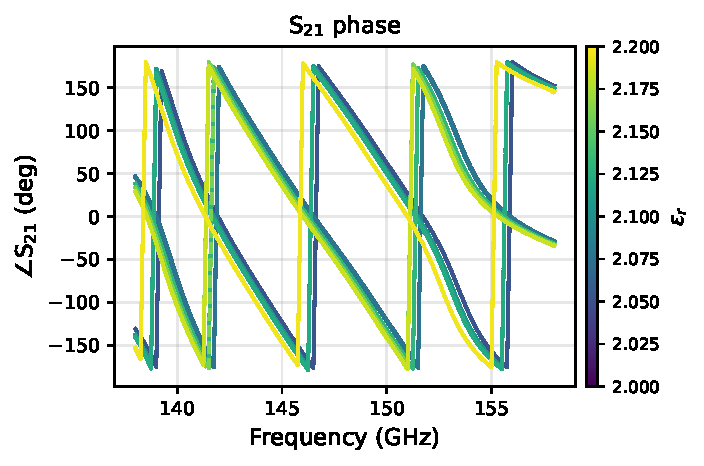
\includegraphics[width=\columnwidth]{figs/fig_s21_phase.pdf}
\caption{DKL surrogate transmission phase $\angle S_{21}$ (degrees). Linear group delay is removed during training via per-$\varepsilon_r$ detrending and restored during inference.}\label{fig:s21phase}
\end{figure}


\begin{figure}[t]
\centering

\includegraphics[width=\columnwidth]{figs/fig_uncertainty_1.pdf}
\caption{S$_{11}$ and S$_{21}$ predictions (left axis) and absolute error in dB (right axis) at $\varepsilon_r = 2.053$ (held-out). Solid: prediction; markers: FEM; dotted: error.}\label{fig:uncert1}
\end{figure}

\begin{figure}[t]
\centering

\includegraphics[width=\columnwidth]{figs/fig_uncertainty_2.pdf}
\caption{S$_{11}$ and S$_{21}$ predictions (left axis) and absolute error in dB (right axis) at $\varepsilon_r = 2.196$ (held-out).}\label{fig:uncert2}
\end{figure}

\section{Pipeline Overview}

Algorithm~\ref{alg:pipeline} summarizes the complete MOR workflow, from FEM data generation to deployment of the trained surrogate with uncertainty quantification.

\begin{algorithm}[t]
\caption{Deep Kernel Learning MOR Pipeline}
\label{alg:pipeline}
\begin{algorithmic}[1]
\Require Permittivity range $[\varepsilon_{\min}, \varepsilon_{\max}]$, frequency range $[f_{\min}, f_{\max}]$, mesh data for bilateral filter
\Ensure Trained DKL surrogate with uncertainty estimates

\Statex \textbf{--- Phase A: Data Generation ---}
\For{each $\varepsilon_r$ value}
    \State Read mesh; assign substrate $\varepsilon_r$; set port BCs
    \State Assemble $\mathbf{S}$, $\mathbf{T}$ matrices via \textsc{AssembleLinear}
    \For{each frequency $f$}
        \State Assemble waveguide port matrices
        \State Solve $(\mathbf{S} - k^2\mathbf{T}) \mathbf{u} = \mathbf{b}$
        \State Extract $\mathbf{S}_{11}$, $\mathbf{S}_{21}$ via modal expansion
        \State Store $(\varepsilon_r, f, S_{11}, S_{21})$
    \EndFor
\EndFor

\Statex \textbf{--- Phase B: Feature Construction ---}
\State Compute harmonic encoding: $\mathbf{x} \gets [\varepsilon_r, f/f_0, \sin\omega, \cos\omega, \sin 2\omega, \cos 2\omega, \sin 3\omega, \cos 3\omega]^\top$
\State $y_1 \gets \operatorname{Re}(S_{11})$, $y_2 \gets \operatorname{Im}(S_{11})$
\State $y_3 \gets \log_{10}|S_{21}|$
\State Fit $S_{21}$ phase slope/intercept per $\varepsilon_r$; compute detrended $y_4$
\State z-score normalize $\mathbf{x}$, $\{y_i\}$ independently

\Statex \textbf{--- Phase C: Training (per channel $i = 1\ldots4$) ---}
\State Initialize FeatureExtractor DNN ($8 \to 1000 \to 1000 \to 500 \to 64$)
\State Initialize ExactGP with product-RBF kernel + GaussianLikelihood

    \hspace*{2em}\textbf{Stage 1 -- DNN warm-start:}
    \State Optimize $\phi$ via MSE loss (100 epochs, $\mathrm{lr}=10^{-3}$)

    \hspace*{2em}\textbf{Stage 2 -- Joint DKL:}
    \State Optimize $\theta$ via $-\log p(\mathbf{y} \mid \mathbf{X}, \theta)$ (500 epochs, $\mathrm{lr}=5\times10^{-3}$, CosineAnnealing)
    \State Evaluate on held-out $\varepsilon_r$ values; store checkpoint

\Statex \textbf{--- Phase D: Inference ---}
\For{each query $(\varepsilon_r, f)$}
    \State Compute harmonic features $\mathbf{x}$; z-score normalize
    \For{each channel $i$}
        \State $\mu_i, \sigma_i \gets \text{ExactGP.predict}(\mathbf{x})$
        \State $\hat{y}_i \gets \text{inverse-normalize}(\mu_i)$
    \EndFor
    \State $S_{11} \gets \hat{y}_1 + j\hat{y}_2$
    \State $|S_{21}| \gets 10^{\hat{y}_3}$; restore phase from detrended $\hat{y}_4$
    \State $S_{21} \gets |\hat{y}_3| \, e^{j\hat{y}_4}$
\EndFor
\State \Return $\hat{S}_{11}$, $\hat{S}_{21}$, $\sigma_{S_{11}}$, $\sigma_{S_{21}}$
\end{algorithmic}
\end{algorithm}

\section{Conclusion}

We have presented a Mixture-of-Experts Deep Kernel Learning framework for millimeter-wave passive device surrogate modeling. The MoE-DKL achieves sub-0.3\% relative error on both S$_{11}$ and S$_{21}$ while providing $6\times 10^2\times$ speedup over FEM with Bayesian uncertainty quantification. Key technical elements include: (1)~harmonic input encoding, (2)~a product-of-RBF base kernel, (3)~targeted output representations per S-parameter, and (4)~a temperature-gated mixture-of-experts architecture that learns specialized feature representations for reflection and transmission physics within a single model.

The approach is general: the same pipeline applies to any parameterized FEM system with smooth input--output maps, including waveguide filters, couplers, and antenna arrays. Future work includes extending the surrogate to support multi-port devices (S$_N$-parameters) with a shared feature extractor, incorporating frequency-rational basis functions through physics-informed kernels, and exploring active learning strategies that query the FEM solver only at points of high predictive uncertainty.

\begin{thebibliography}{00}

\bibitem{quarteroni2015reduced}
A.~Quarteroni, A.~Manzoni, and F.~Negri, \textit{Reduced Basis Methods for Partial Differential Equations}. Springer, 2015.

\bibitem{rozza2008efficient}
G.~Rozza, D.~B.~P.~Huynh, and A.~T.~Patera, ``Reduced basis approximation and a posteriori error estimation for affinely parametrized elliptic coercive partial differential equations,'' \textit{Arch. Comput. Methods Eng.}, vol.~15, no.~3, pp.~229--275, 2008.

\bibitem{gustavsen1999rational}
B.~Gustavsen and A.~Semlyen, ``Rational approximation of frequency domain responses by vector fitting,'' \textit{IEEE Trans. Power Del.}, vol.~14, no.~3, pp.~1052--1061, 1999.

\bibitem{burrascano1998learning}
P.~Burrascano, S.~Fiori, and M.~Mongiardo, ``A review of artificial neural networks for waveguide filter optimization,'' \textit{Int. J. RF Microw. Comput.-Aided Eng.}, vol.~8, no.~5, pp.~407--421, 1998.

\bibitem{feng2018neural}
F.~Feng, C.~Zhang, J.~Ma, and Q.-J.~Zhang, ``Parametric modeling of microwave components using adjoint neural networks and pole-residue transfer functions with EM sensitivity analysis,'' \textit{IEEE Trans. Microw. Theory Tech.}, vol.~66, no.~4, pp.~1755--1768, 2018.

\bibitem{swiler2011gaussian}
L.~P.~Swiler and T.~L.~Paez, ``Gaussian process emulators for simulating complex physics models,'' Sandia National Laboratories, Tech. Rep. SAND2011-2693, 2011.

\bibitem{wilson2016deep}
A.~G.~Wilson, Z.~Hu, R.~Salakhutdinov, and E.~P.~Xing, ``Deep kernel learning,'' in \textit{Proc. 19th Int. Conf. Artificial Intelligence and Statistics (AISTATS)}, 2016, pp.~370--378.

\bibitem{bornemann2010waveguide}
J.~Bornemann, U.~Rosenberg, and S.~Amari, \textit{Planar Microwave Engineering: A Practical Guide to Theory, Measurement, and Circuits}. Cambridge University Press, 2010.

\bibitem{jin2015finite}
J.-M.~Jin, \textit{The Finite Element Method in Electromagnetics}, 3rd~ed. Wiley, 2015.

\bibitem{rasmussen2006gaussian}
C.~E.~Rasmussen and C.~K.~I.~Williams, \textit{Gaussian Processes for Machine Learning}. MIT Press, 2006.

\bibitem{kay1998fundamentals}
S.~M.~Kay, \textit{Fundamentals of Statistical Signal Processing: Estimation Theory}. Prentice Hall, 1998.

\bibitem{ntibarikure2012}
L.~Ntibarikure, G.~Pelosi, and S.~Selleri, ``Efficient harmonic balance analysis of waveguide devices with nonlinear dielectrics,'' \textit{IEEE Microw. Wireless Compon. Lett.}, vol.~22, no.~5, pp.~221--223, 2012.

\bibitem{pyfes2025}
L.~Ntibarikure, ``pyFES: Python Finite Element Software for electromagnetics,'' 2025. [Online]. Available: \url{https://github.com/ntilau/pyFES}

\end{thebibliography}

\end{document}
